%% uctest.tex 11/3/94
%% Copyright (C) 1988-2004 Daniel Gildea, BBF, Ethan Munson.
%
% This work may be distributed and/or modified under the
% conditions of the LaTeX Project Public License, either version 1.3
% of this license or (at your option) any later version.
% The latest version of this license is in
%   http://www.latex-project.org/lppl.txt
% and version 1.3 or later is part of all distributions of LaTeX
% version 2003/12/01 or later.
%
% This work has the LPPL maintenance status "maintained".
% 
% The Current Maintainer of this work is Daniel Gildea.

\documentclass[11pt]{ucthesis}
\def\dsp{\def\baselinestretch{2.0}\large\normalsize}
\dsp

\usepackage{graphicx}
 \usepackage{subfigure}% subcaptions for subfigures
 \usepackage{lettrine}% dropped capital at beginning of paragraph
 \usepackage{hyperref}% embedding hyperlinks [must be loaded after dropping]
 \usepackage{amsmath}
 \usepackage{color}
\begin{document}

% Declarations for Front Matter

\title{Modeling and Control of Active Twist Aircraft}
\author{Nicholas Bryan Cramer}
\degreeyear{2017}
\degreemonth{March}
\degree{DOCTOR OF PHILOSOPHY}
\chair{Professor Mircea Teodorescu}
\committeememberone{Professor Ricardo Sanfelice}
\committeemembertwo{Dr. Sean Swei}
\numberofmembers{3} %% (including chair) possible: 3, 4, 5, 6
\deanlineone{Dean Tyrus Miller}
\deanlinetwo{Vice Provost and Dean of Graduate Studies}
\deanlinethree{}
\field{Computer Engineering}
\campus{Santa Cruz}

\begin{frontmatter}

\maketitle
\copyrightpage

\tableofcontents
\listoffigures
\listoftables

\begin{abstract}
Theses have elements.  Isn't that nice?

\end{abstract}

\begin{dedication}
\null\vfil
{\large
\begin{center}
To ,\\\vspace{12pt}

\end{center}}
\vfil\null
\end{dedication}


\begin{acknowledgements}
I want to thank
\end{acknowledgements}

\end{frontmatter}

%%%%%%%%%%%%%%%%%%%%%%%%%%%%%%%%%%%%%%%%%%%%%%%%%%%%%%%%%%%%%%%%%%%%%%%%%%%
\chapter{Introduction}

\section{Motivation}
Demand for commercial air travel has increased at an steady rate of $9\%$ annual growth rate of passenger and freight traffic globally over the past three decades. \cite{upham2003environmental} With the continued increase in demand for air travel the ramifications of air travel must be addressed. These range from health concerns to ever increasing $CO_2$ emissions. It is expected that between 1995 and 2050 the contribution of $CO_2$ from air travel will in increase by a factor of 36 which is why air travel and its efficiency are heavily discussed in climate change policy. \cite{olsthoorn2001carbon} While air travel has it's downsides it is also a critical component for trade \cite{smith2001world}, regional developments \cite{marazzo2010air}, and intercultural communications \cite{adey2007flying}. With air travels critical role in financial and social institutions it is unreasonable to expect that anything less and a holistic solution of technological and policy advancement could appropriately address the salient issues associated with it.

Increased aircraft efficiency is typically achieved either by a reduction of weight or and increase of aerodynamic efficiency. In the industry the most common production level approach is to reduce weight through the use of composites. For example Boeing's 787 Dreamlines which was able to achieve a 20\% weight reduction by using carbon fiber plastic composites. \cite{hale2006boeing} On the other end of the spectrum the aerospace community has been investigating the use of morphing aircraft to increase the aerodynamic efficiency through the use of shape morphing.\cite{barbarino2011review,kuzmina2002review,sofla2010shape} Shape morphing can be described as the ability of an aircraft to change some form of its geometry. There are very few limitation of what can be considered ``shape morphing'' other than the fact that traditional hinged flaps/slats are not sufficient changes in the aircraft geometry to be counted. Figure \ref{fig:airGeo} shows the general range of aircraft geometries that can be adjusted for reference. 

\begin{figure}[h]
\centering
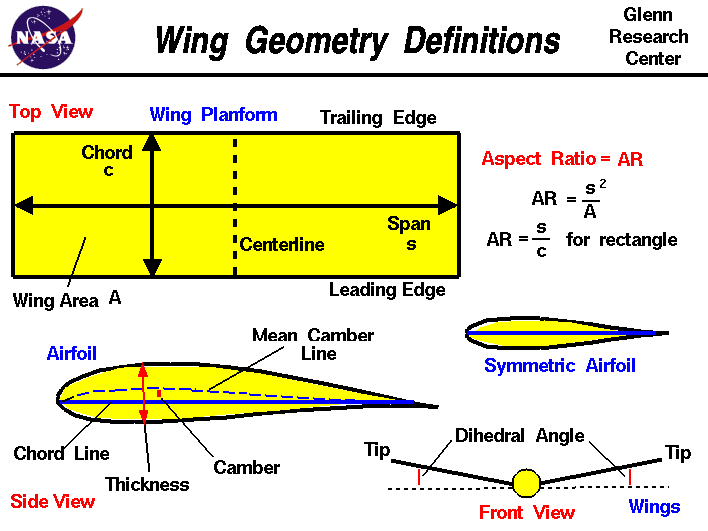
\includegraphics[width=0.75\linewidth]{./Figures/AircraftGeom.png}
\caption{General definitions of aircraft geometries, provided by NASA Glenn Research Center}
\label{fig:airGeo}
\end{figure}

Shape morphing typically achieves the increase in aerodynamic efficiency by changing the aircraft geometry to become more optimal at various flight conditions. Typical fixed wing aircraft are designed to have maximum efficiency around their nominal cruise conditions, which necessarily results in the design being sub-optimal at other flight conditions. In theory the aircraft should spend the vast majority of it's flight time at its nominal cruise condition but due to things like weather, airspace congestion, and distance of flight this is not always true and shape morphing can help address this problem.  

There are four major challenges associated with making shape morphing a viable technology for the industry, distributed high-power density actuation, structural mechanization, flexible skins, and control law development. \cite{reich2007introduction} Of these primary challenges we will be addressing the control law development but the linkage between all of these challenges will be evident. I will specifically be focusing on the development of reasonable models, control and capability analysis of an active twist aircraft. Wing twist is defined as the angle that the wing tip is compared to the angle that the wing meets the aircraft body as shown in Figure \ref{fig:twist}. Wing twist was selected because it is capable of generating many interesting and potentially important phenomena for increased efficiency.

\begin{figure}[h]
\centering
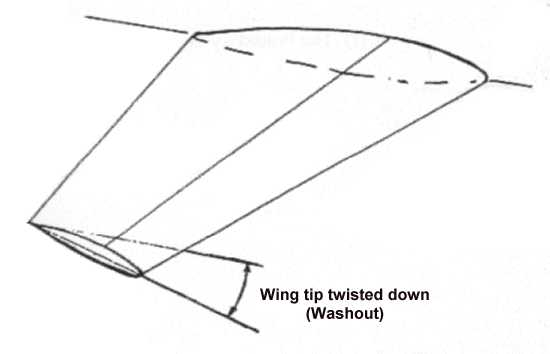
\includegraphics[width=0.75\linewidth]{./Figures/twist.jpg}
\caption{Definition of wing twist, where the tip of the wing is twisted at an angle different than the one that the wing meets the plane body at}
\label{fig:twist}
\end{figure}

\section{Applications}
Our motivation example focused primarily on commercial aircraft but the application space for this research can be broken down into three area, where commercial aircraft are but one part.
\begin{itemize}
\item Commercial Aviation - The commercial aviation sector was touched on above but effective control of active twist could have a direct and immediate impact on this field. A very effective use of wing twist could be the creation of active twisting winglits that can be trimmed to optimal wash out of various flight regimes. This could provide significant performance increases during take-off and landing.
\item Military Aircraft - The military has a desire to have an aircraft that is flexible to a multitude of missions. The use of active twist technology would allow for more efficient vehicles and longer flights but more crucially would increase the performance envelope of the aircraft. It could be especially important as an enabling technology for other high efficiency designs such as blended body and flying wings where the minimum stability margin of the aircraft can be catastrophically affected by the discontinuities that come from traditional flaps.
\item Unmanned Aerial Vehicles (UAVs) - UAVs have a lot of promise as means of delivery or inspection but one of the primary problems is that the rotocopter set-up that is ideal for these missions has sever longevity issues while the fixed wing variant need long ranges to take off and land and are difficult to loiter in the same spot. The active twist technology could help by decreasing the loiter speed and loiter radius of the UAV while also decreasing the range necessary to take off and land.
\item High Altitude Long Endurance (HALE) Aircraft - Active twist for HALE aircraft have many of the same advantages as commercial aviation but they also have a distinct advantage of not typically having passengers. This means that it is possible for the HALE to take advantage of some of the aerodynamic efficiency gains of active that can be seen in flapping flight that would be untenable for passengers.
\end{itemize}

\section{Contributions of this Work}
In this work we try to take a holistic approach to the design and analysis of the active twist controllers as such there are some varied contributions to the field which are listed below.

\begin{itemize}
\item Development of an aeroelastic simulation method that is specifically tailored to the targeted operating regime. 
\item Design of wind tunnel tests to access the broader capabilities of the technology and validate the simulation.
\item Creation of decentralized control expanding on the work of Siljak \cite{siljak2011decentralized} to address the issues associated with overlapping decentralized control.
\item Expansion of the concept of the transfer matrix method as a means of control centered modeling and decentralized structural stabilization.
\item Explored the use of aerodynamic database for structural state estimation and inner loop active twist control.
\end{itemize}

%%%%%%%%%%%%%%%%%%%%%%%%%%%%%%%%%%%%%%%%%%%%%%%%%%%%%%%%%%%%%%%%%%%%%%%%%%%
\chapter{Background}
\section{Aeroelastic Modeling}

\section{Morphing Wings}
Morphing wings as a means of control is an intuitive and readily understandable means of controlling an aircraft. In our daily life we often see birds flying and their primary mechanism of motion control is changing the shape of their wings. Not surprisingly then the first attempt at roll control was done via wing warping during the Wright brothers first flight. \cite{friswell2009prospects} The use of compliant wing morphing mechanisms quickly fell out of favor it seems likely this was due to the rise of the structural shell mechanism, for which the shell of the aircraft became the primary structural component. While aircrafts still used truss structures like that found in the Wright brother's plane the weight was reduced dramatically by having the shell bare the load. \cite{weisshaar2011aerospace} It seems likely that the additional engineering effort to make the shell compliant to actuation while resisting aeroloading and the relative ease at which traditional control surfaces could be manufactured resulted in the dormancy of morphing wing research.

Work on compliant morphing wings resumed in the 1980's with Air Force Research Laboratory's (AFRL) the Active flexible wing (AFW) technology project that was using traditional control surfaces to shape a compliant wing. \cite{miller1988active} This was eventually followed by the ``PARTI'' \cite{pinkerton1996controlled} and DAPRA's Smart Wing Project \cite{kudva2001overview} who used smart materials as a means of actuation for the morphing airfoil, irreversibly linking the morphing wing research to the continued development of smart materials. With the turn of the century research in morphing aircraft exploded, in the next few sections we will explore some of the more relevant morphing wing research.

\subsection{Camber Morphing}
Changing the camber of an airfoil is probably the most researched area of morphing wing research. This is because the dramatic changes that the camber can have on the aerodynamic performance. 

One of the most successful Small Business Innovation Research (SBIR) in recent memory has been FlexSys which created an variable camber trailing edge for  wings\cite{kota2009mission} and rotors\cite{kota2008adaptive}. The FlexSys system uses a underlying compliant mechanism to control the structural deformation of the airfoil and therefore the camber with a simple rotary actuator. This structure encourages a reduction of stress concentrations  and the weight  of joints while minimizing backlash. The interface between the stiff wing and the compliant trailing edge is an elastomer membrane. FlexSys was able to demonstrate the effectiveness of their variation of the camber morphing through model test flight and are currently performing full scale slight systems both of which have yielded positive results. 

The spiritual successor at AFRL to the ARW program is the AFRL Variable Camber Compliant Wing (VCCW) which shares a lot of similarities to the FlexSys system. The VCCW is focused on optimization of the variable camber design by combining the the leading and trailing edge mechanism, eliminating the need for stretchable skin, while minimizing the energy consumption. The VCCW has been exhaustively studied prior to flight testing via bench top testing and simulations \cite{miller2015fluid} as well as wind tunnel testing \cite{zientarski2015wind} both showing the expected performance increases. 

The final camber morphing project that I will highlight is NASA and Boeing's Variable Camber Continuous Trailing Edge Flap (VCCTEF). The VCCTEF bears some similarities to the AFW project in that it is using the the flaps to control the aerodynamic forces and the resultant wing shaping. This is achieved via numerous trailing edge flaps that changed the airfoil camber and are attached to each other via and elastomer filling. The flap actuation is achieved with a slow large displacement using Shape Memory Alloy (SMA) and faster electric drive motors for the outboard flap.\cite{urnes2013mission} The configuration of the actuator results in actuation constraints that much be taken into account. \cite{swei2014aeroelastic} Of the camber morphing technologies presented here the the VCCTEF project is one of the only ones that committed a significant effort to investigating the control of the aircraft\cite{nguyen2012aeroelastic} though additional validation has not been completed beyond simulations.
\subsection{Flapping Flight}
\subsection{Active Twist}

\section{Control}
\subsection{Aeroelastic Control}
\subsection{Decentralized Control}

%%%%%%%%%%%%%%%%%%%%%%%%%%%%%%%%%%%%%%%%%%%%%%%%%%%%%%%%%%%%%%%%%%%%%%%%%%%
\chapter{Modeling}
\section{Structural Modeling}
\subsection{Galerkin Method}
\subsection{Transfer Matrix Method}

\section{Aerodynamics}

\section{Aeroelastic}

%%%%%%%%%%%%%%%%%%%%%%%%%%%%%%%%%%%%%%%%%%%%%%%%%%%%%%%%%%%%%%%%%%%%%%%%%%%
\chapter{Testing and Validation}
\section{Wind Tunnel Testing}
\section{Results and Validation}

%%%%%%%%%%%%%%%%%%%%%%%%%%%%%%%%%%%%%%%%%%%%%%%%%%%%%%%%%%%%%%%%%%%%%%%%%%%
\chapter{Control}
\section{Structural Stability Control of Lattice Structure}

\section{Active Twist Aircraft Control}

%%%%%%%%%%%%%%%%%%%%%%%%%%%%%%%%%%%%%%%%%%%%%%%%%%%%%%%%%%%%%%%%%%%%%%%%%%%
\chapter{Conclusion}
\section{Summary}
\section{Future Works}

\nocite{*}
\bibliographystyle{plain}
\bibliography{thesis}

\end{document}
